\documentclass{beamer}
\usetheme[faculty=econ]{fibeamer}

\usepackage[utf8]{inputenc}
\usepackage[francais]{babel}
\usepackage[T1]{fontenc}
\usepackage{xcolor}

\lstset{
  language=Java,                
  basicstyle=\scriptsize,
  escapeinside={*@}{*@},
  frame=single,
  xleftmargin=2mm,
  xrightmargin=2mm,
  keepspaces=true,
  tabsize=2
}

\newcounter{ctr1}
\title[]{\Large{Développement d'applications modulaires en Java}}
\author[C. Tibermacine]{\large{Chouki~Tibermacine}\\
\small{Chouki.Tibermacine@umontpellier.fr}}
%\institute{Polytech Montpellier}
\date{}

\begin{document}

\begin{frame}
\titlepage
\begin{flushright}

\includegraphics[width=3.5cm]{figs/polytech.png}
\end{flushright}
\end{frame}

\begin{frame}
  \frametitle{Plan de l'ECUE}
\begin{enumerate}
\item (Rappels sur le) Développement d'applications Web avec Java
\item Modulariser les applications Java avec Spring
\item Bien structurer une application Web avec Spring MVC
\item Auto-configurer une application Web avec Spring Boot
\item Sécuriser une application Web avec Spring Security
\item Gérer des données massives avec Apache Kafka et Spring
\item Tester une application Web Spring
\item Écrire des applications Web (API) réactives avec Spring WebFlux
\end{enumerate}
\end{frame}


\begin{frame}
  \frametitle{Plan de l'ECUE}
\begin{enumerate}
\item (Rappels sur le) Développement d'applications Web avec Java
  {\color{gray}{
	\item Modulariser les applications Java avec Spring
  	\item Bien structurer une application Web avec Spring MVC
  	\item Auto-configurer une application Web avec Spring Boot
  	\item Sécuriser une application Web avec Spring Security
  	\item Gérer des données massives avec Apache Kafka et Spring		
  	\item Tester une application Web Spring
  	\item Écrire des applications Web (API) réactives avec Spring WebFlux}}
  \end{enumerate}
\end{frame}

\AtBeginSection[]{% Print an outline at the beginning of sections
  \begin{frame}<beamer>
    \frametitle{Plan du cours}
    % \frametitle{Outline}
    \tableofcontents[currentsection]
    % \tableofcontents
  \end{frame}}

\AtBeginSubsection[]{% Print an outline at the beginning of sections
  \begin{frame}<beamer>
    \frametitle{Plan du cours}
    % \frametitle{Outline}
    \tableofcontents[currentsubsection]
    % \tableofcontents
  \end{frame}}

\section{Introduction à la programmation Web avec Java}

\begin{frame}
  \frametitle{Qu'est-ce qu'une application Web~?}
  \begin{itemize}
  \item Un ensemble de ressources (pages et services Web) déployé sur un serveur accessible via le protocole HTTP
  \item Des requêtes HTTP parviennent au serveur Web et sont redirigées
    vers l'application:\\
    \texttt{http://{\color{green}someserver}/{\color{red}myapp}/endpoint}
  \item Le serveur renvoie des réponses HTTP avec du :
  \begin{itemize}
  \item contenu statique : pages HTML, images, scripts clients, ...
  \item contenu généré dynamiquement par des programmes serveurs
    \end{itemize}
  \end{itemize}
\end{frame}

\begin{frame}
  \frametitle{Déploiement d'une application Web Java}
  \begin{itemize}
  \item Déploiement fait simplement en copiant le contenu de
    l'application dans un dossier particulier du serveur Web
    \begin{itemize}
    \item Dossier \texttt{webapps/} du répertoire d'installation de Tomcat
      \begin{block}{Serveur Web Tomcat}
        \begin{itemize}
        \item Télécharger Tomcat v10: \url{https://tomcat.apache.org/download-10.cgi}
        \item Décompresser l'archive
        \item Démarrer le serveur en utilisant le script
          \texttt{catalina} qui se trouve dans le dossier
          \texttt{bin/} de l'archive décompressée (\texttt{catalina.sh start})
        \item Page d'accueil du serveur Web accessible sur:
          \url{http://localhost:8080}
          \end{itemize}
    \end{block}
    \end{itemize}
  \end{itemize}
\end{frame}

\begin{frame}
  \frametitle{Structure d'une application Web Java}
  \begin{itemize}
  \item Une structure standard pour le contenu d'une app: ouvrez le sous-dossier \texttt{examples/} de \texttt{webapps/} dans Tomcat
  \item A la racine du dossier d'une application, des fichiers HTML,
    images, des scripts client ou serveur, ...
  \item On trouve aussi un dossier \texttt{WEB-INF/}, qui comporte:
    \begin{itemize}
    \item configuration de l'application dans \texttt{web.xml} (voir plus loin)
    \item classes qui composent l'application
    \item bibliothèques utilisées par l'application
    \end{itemize}
  \item L'application peut exister sous la forme d'une archive ZIP
    (fichier .war : \textit{Web ARchive}), avec la même structure que ci-dessus
  \end{itemize}
\end{frame}    

\begin{frame}
  \frametitle{Administrer le déploiement d'applications}
  \begin{itemize}
  \item Interface Web~: \url{http://localhost:8080/manager/html}
  \item Cela nécessite une authentification
  \item Ajouter d'abord un utilisateur gestionnaire (\textit{manager user}) :
    \begin{itemize}
    \item Éditer le fichier \texttt{tomcat-users.xml} du dossier
      \texttt{conf/} de l'install Tomcat
    \item Ajouter la ligne suivante~:\\
      \texttt{<user username="bob" password="LoveAlice4Ever;" roles="manager-gui"/>}
    \end{itemize}
  \item On peut démarrer, arrêter, recharger-sans-arrêter, ... les
    applications existantes
  \item On peut déployer une nouvelle app (un WAR, par exemple)
  \end{itemize}
\end{frame}

\section{Programmes serveurs Web Java}

\subsection{Servlets}
\begin{frame}
  \frametitle{Notions de base}
  \begin{itemize}
  \item Programmes serveurs : \textit{Servlets} (avec ça, on peut tout faire) et \textit{Jakarta Server Pages} (ex-\texttt{JavaServer Pages}) -- JSP
  \item Il existe de nombreux frameworks construits au dessus de ces notions
  \item Exemples de frameworks : Struts \& Spring (vu dans ce cours)
  \end{itemize}
\end{frame}

\begin{frame}
  \frametitle{Interface implémentée par les servlets}
      \begin{tikzpicture}[overlay,remember picture]
        \node[anchor=center,xshift=0pt,yshift=-45pt]
        at (current page.center) {
          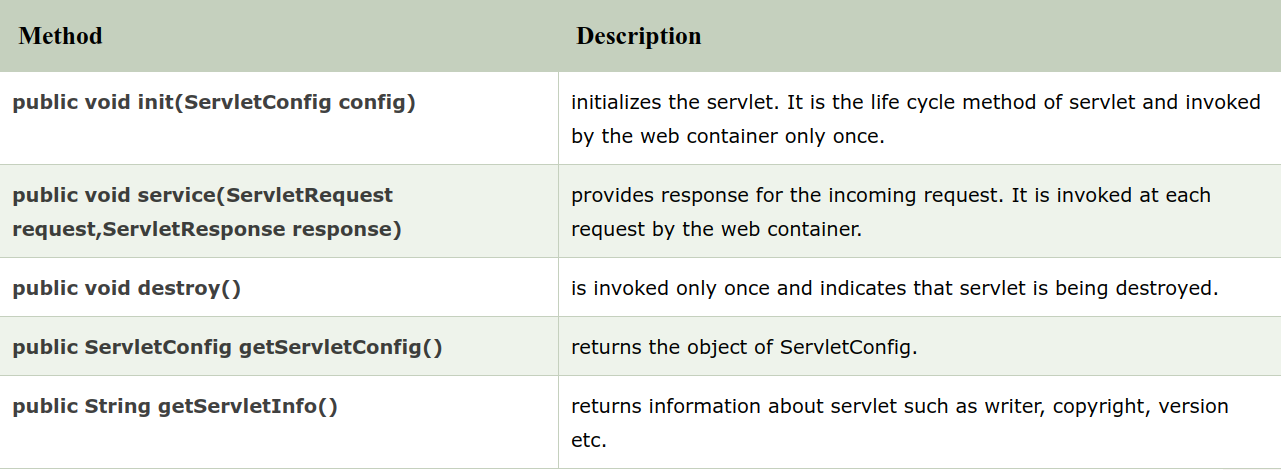
\includegraphics[width=12cm]{img/ServletInterface.png}
        };
      \end{tikzpicture}
      \begin{itemize}
      \item Interface \texttt{javax.servlet.Servlet} (dans les versions récentes de l'API, 4.0+, c'est \texttt{jakarta.servlet.Servlet} -- remplacer partout \texttt{javax.servlet} par \texttt{jakarta.servlet})
      \vspace{4.5cm}
    \item Interface indépendante d'un protocole (HTTP, FTP, ...)
      \end{itemize}
\end{frame}

\begin{frame}
  \frametitle{Servlets}  
  \begin{itemize}
  \item L'interface précédente peut être implémentée directement, mais
    c'est long à faire
  \item La bibliothèque qui vient avec le serveur Web (dossier
    \texttt{lib/}) fournit des classes ``\textit{Helper}''
  \item Parmi ces classes, nous retrouvons \texttt{GenericServlet}
    (une classe abstraite) et \texttt{HttpServlet}
  \end{itemize}
\end{frame}

\begin{frame}
  \frametitle{Classe \texttt{HttpServlet}}
      \begin{tikzpicture}[overlay,remember picture]
        \node[anchor=center,xshift=0pt,yshift=-10pt]
        at (current page.center) {
          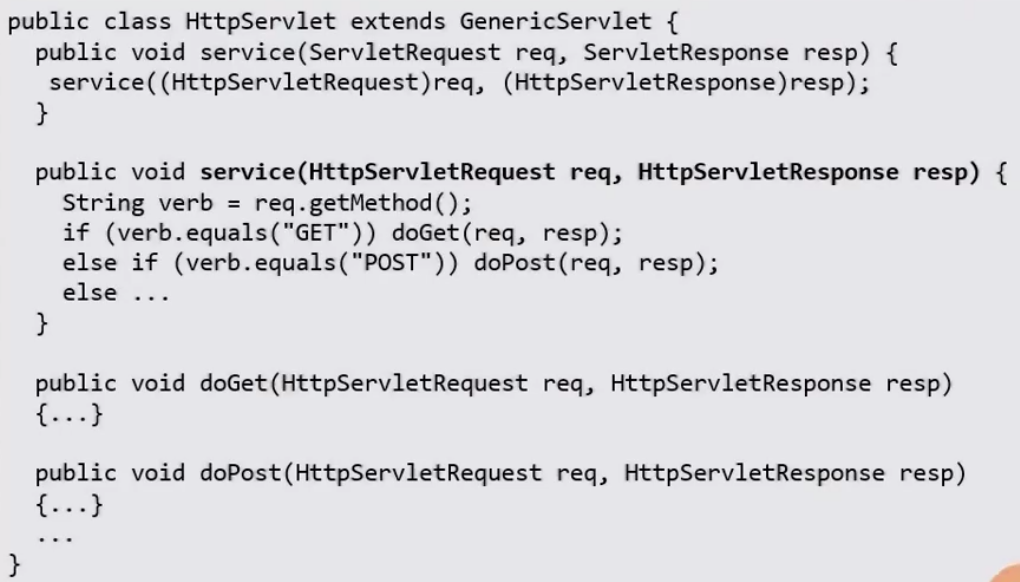
\includegraphics[width=12cm]{img/HttpServlet.png}
        };
      \end{tikzpicture}
\end{frame}

\begin{frame}
  \frametitle{Exemple de servlet}
  \begin{tikzpicture}[overlay,remember picture]
    \node[anchor=center,xshift=0pt,yshift=0pt]
    at (current page.center) {
      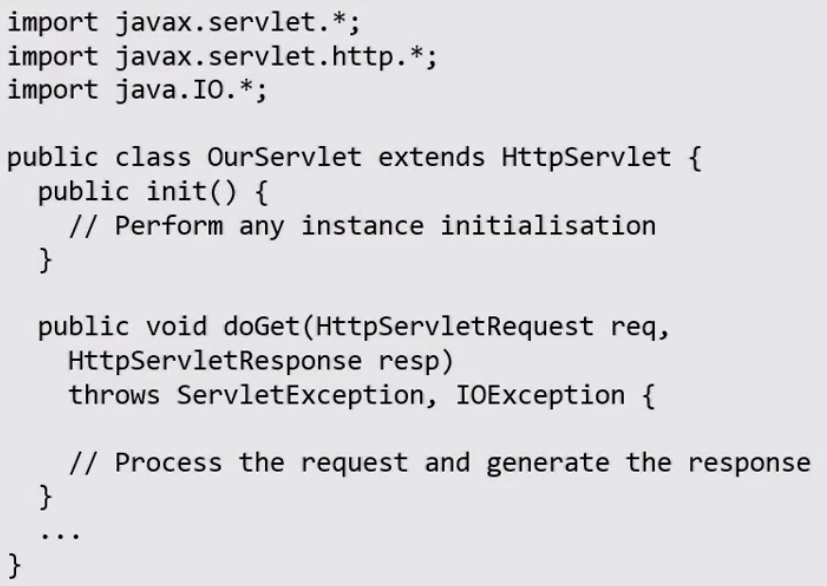
\includegraphics[width=9cm]{img/OurServlet.png}
    };
  \end{tikzpicture}
  \begin{itemize}
    \vspace{5.5cm}
  \item On redéfinit ces méthodes dans une app Web: \texttt{doGet()},
    \texttt{doPost()}, \texttt{doPut()}, ...
  \end{itemize}
\end{frame}

\begin{frame}
  \frametitle{Exemple de servlet (\textit{Servlet Mapping})}
  \begin{tikzpicture}[overlay,remember picture]
    \node[anchor=center,xshift=30pt,yshift=-20pt]
    at (current page.center) {
      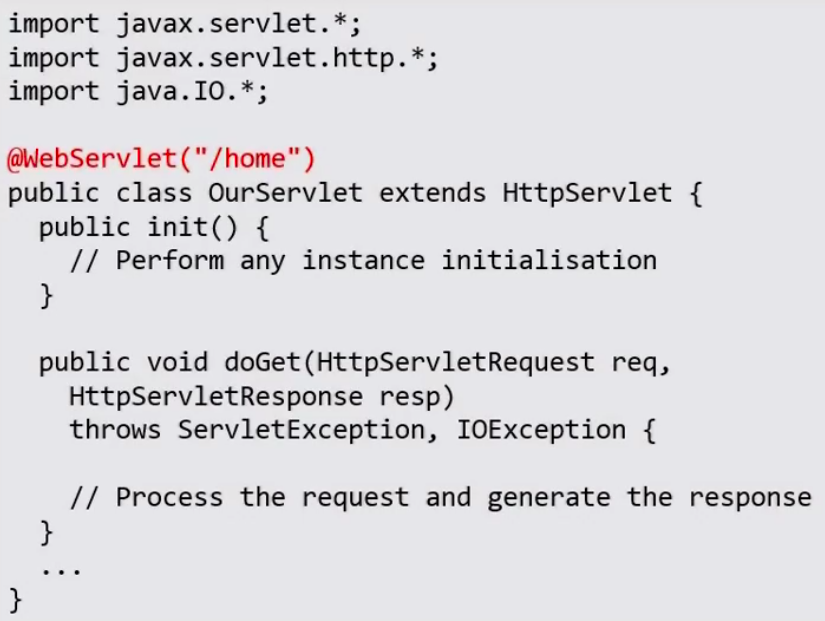
\includegraphics[width=7cm]{img/OurServlet2.png}
    };
  \end{tikzpicture}
  \begin{itemize}
    \item Comment le serveur peut identifier quelle servlet répond à une
    requête~?  
    \item[]\vspace{4cm}
	\item Importer l'annotation \texttt{@WebServlet} de \texttt{javax.servlet.annotation} (\texttt{jakarta.servlet...})
  \end{itemize}
\end{frame}

\begin{frame}
  \frametitle{A vos claviers}

  \begin{itemize}
  \item Écrire une servlet qui répond à une requête HTTP Get avec le
    message ``\textit{Hello Java Web World!}''
    \item D'abord, faire cela à la main (étapes élémentaires)~:
    \begin{enumerate} 
    	\item copier la classe qui se trouve sur le dépôt Git et la compiler, en ajoutant dans le CLASSPATH le jar \texttt{servlet-api.jar} qui se trouve dans le dossier \texttt{lib/} de Tomcat,
    	\item  créer un dossier simpleapp/ dans webapps/, créer dedans un dossier WEB-INF/classes/ et mettre le .class dans ce dossier, 
    	\item démarrer Tomcat, en allant dans le dossier bin/ de Tomcat et en tapant la commande ./catalina.sh start (changer les droits sur le fichier .sh si celui-ci n'est pas exécutable)
    	\item Dans votre navigateur, aller à~: \url{http://localhost:8080/simpleapp/home}
    \end{enumerate}
  \item Ensuite, utiliser IntelliJ IDEA pour éditer le code et Gradle pour construire et déployer le projet (voir prochaines diapos)
  \end{itemize}
\end{frame}

\begin{frame}
	\frametitle{A vos claviers -suite-}
	
	\begin{itemize}
		\item Installer Gradle (dans les systèmes Unix, vous pouvez installer SDKMAN! d'abord: \url{https://sdkman.io/})
		\item Ceux qui ne connaissent pas Gradle, c'est un système de build, comme Maven --même structure pour les projets, mais pour les scripts de build on utilise un DSL (\textit{Domain Specific Language}) Groovy ou Kotlin et non XML
		\item Tester votre installation de Gradle sur un terminal : \texttt{gradle -v}
		\item Initialiser un projet Java simple : \texttt{gradle init}
		\begin{itemize}
			\item Choisir comme type de projet  ``\texttt{2: application}"
			\item Choisir comme langage d'implémentation ``\texttt{3: Java}"
			\item Choisir comme DSL pour le script de build : ``\texttt{2: Kotlin}"
			\item Choisir l'option par défaut pour le framework de Test (\texttt{JUnit 4})
			\item Donner un nom à votre projet: SimpleApp et donner un nom de package: \texttt{fr.polytech.mtp.ig5.iaw2.c1}
		\end{itemize} 
\end{itemize}
\end{frame}

\begin{frame}
\frametitle{A vos claviers -suite-}

\begin{itemize}
	\item Que s'est-il passé ? inspecter le dossier courant et ouvrez le fichier \texttt{build.gradle.kts}
	\item Expliquer les lignes de ce fichier
	\item Où se trouve la classe principale de l'application~?
	\item Lister les tâches possibles à faire dans ce projet : \texttt{gradle tasks}
	\item Exécuter votre app: \texttt{gradle run}
	\item Ceci déclenchera plusieurs tâches. Identifier ces tâches
	\item[*]Utiliser gradle run -i
	\end{itemize}
\end{frame}

\begin{frame}[fragile]
	\frametitle{A vos claviers -- transformer le projet en app Web}
	
	\begin{itemize}
		\item Éditer le script de build, \texttt{build.gradle.kts} pour y mettre le contenu suivant~:
		\footnotesize
\begin{lstlisting}
plugins {
	id "war"
	id "org.gretty" version "3.0.6" // ou version plus
							// recente pour l'API 4.0+ des servlets
}		
repositories {
	mavenCentral()
}
dependencies {
	providedCompile("javax.servlet:javax.servlet-api:4.0.1")
	testImplementation("junit:junit:4.12")
}	
\end{lstlisting}
		\normalsize
		\item[] Le plugin gretty permet d'installer et démarrer un serveur Web Tomcat (Fondation Apache) ou Jetty (Fondation Eclipse)

	\end{itemize}
\end{frame}

\begin{frame}
	\frametitle{A vos claviers -- transformer le projet en app Web}
	
	\begin{itemize}
		\item Ajouter un dossier \texttt{webapp/} sous \texttt{src/main}
		\item Ajouter dans ce dossier une page Web dans laquelle est affichée la phrase "Hello World!"
		\item Changer de wrapper Gradle (pour utiliser une version standard de Gradle) :
	$gradle~wrapper~--gradle-version=6.6.1$
	\item Lancer le build~: \texttt{gradlew build}
	\item Démarrer le serveur Web Jetty et y déployer votre app~:\\
	\texttt{gradlew jettyStart}
	\item Aller dans votre navigateur Web à la page~:\\
	\url{http://localhost:8080/SimpleApp}\\
	où \texttt{SimpleApp} est le nom de votre projet
	\end{itemize}
\end{frame}

\begin{frame}
	\frametitle{A vos claviers -- transformer le projet en app Web}
	
	\begin{itemize}
		\item Ajouter dans la page Web un formulaire pour saisir le nom d'un utilisateur
		\item Quand le formulaire est soumis, une servlet renvoie le message ``Hello" suivi du nom de l'utilisateur
		\begin{itemize}
			\item L'attribut \texttt{action} du formulaire doit avoir comme valeur ``\texttt{home}"
			\item La servlet est placée dans le dossier \texttt{src/main/java} (vous pouvez simplement modifier la classe \texttt{App} créée précédemment)
			\item Pour récupérer la valeur d'un champ de formulaire dans la servlet~: (le \textit{name} du champ est ``\texttt{name}'')\\
			\texttt{String name = request.getParameter("name");}
		\end{itemize}
		\item Tester l'application
		\item Arrêter le serveur ...		
	\end{itemize}
\end{frame}

\begin{frame}
	\frametitle{Servlet Mappings -- routes des requêtes HTTP}
	\begin{tikzpicture}[overlay,remember picture]
		\node[anchor=center,xshift=0pt,yshift=-15pt]
		at (current page.center) {
			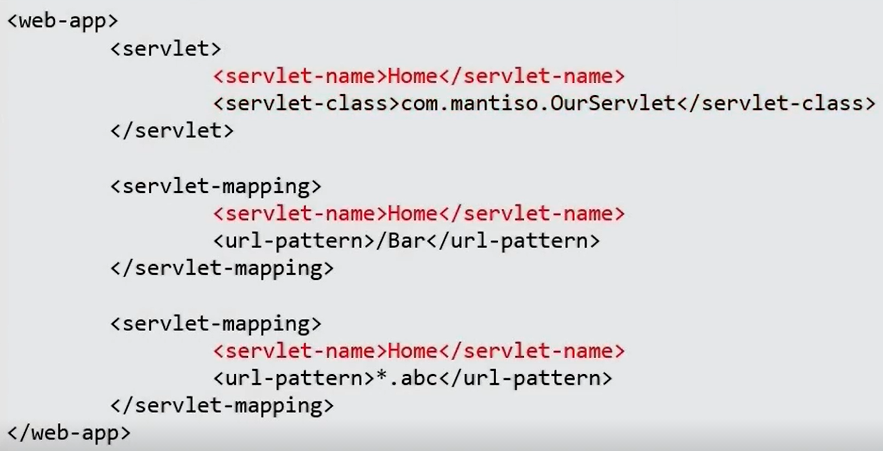
\includegraphics[width=8.5cm]{img/ServletMappings.png}
		};
	\end{tikzpicture}
	\begin{enumerate}
		\item A l'ancienne (fichier \texttt{WEB-INF/web.xml} dans  \texttt{webapp/})~:
		\vspace{4.5cm}
	
\item Avec les annotations~:\\
\footnotesize
\texttt{@WebServlet(urlPatterns={"hello","*.do"})}
\normalsize
\end{enumerate}
\end{frame}

\begin{frame}
	\frametitle{Objet \texttt{HttpServletRequest}}
	\begin{tikzpicture}[overlay,remember picture]
		\node[anchor=center,xshift=0pt,yshift=-15pt]
		at (current page.center) {
			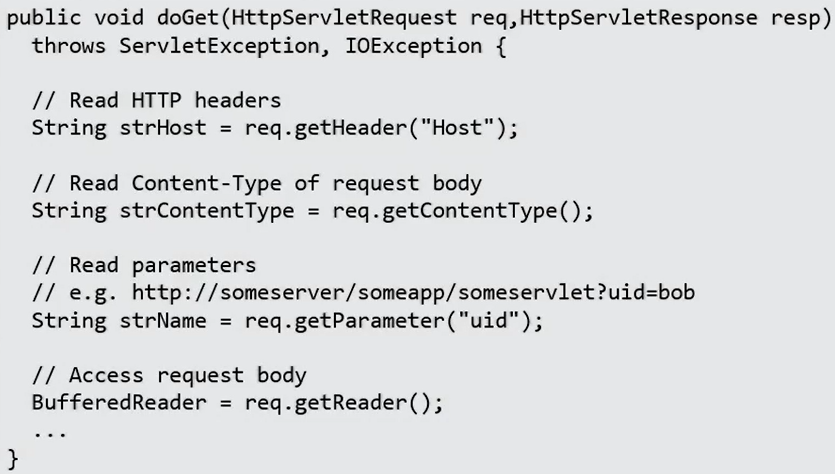
\includegraphics[width=11.5cm]{img/HttpServletRequest.png}
		};
	\end{tikzpicture}
\end{frame}

\begin{frame}
	\frametitle{Objet \texttt{HttpServletResponse}}
	\begin{tikzpicture}[overlay,remember picture]
		\node[anchor=center,xshift=0pt,yshift=-15pt]
		at (current page.center) {
			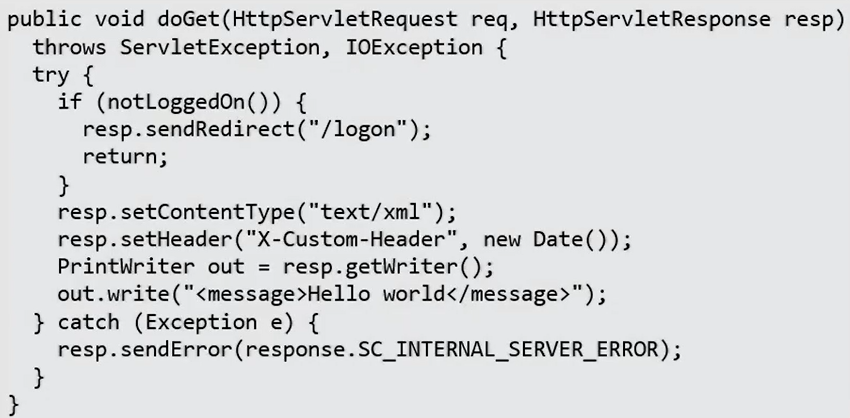
\includegraphics[width=11.5cm]{img/HttpServletResponse.png}
		};
	\end{tikzpicture}
\end{frame}

\begin{frame}
	\frametitle{Initialiser une servlet}
	\begin{tikzpicture}[overlay,remember picture]
		\node[anchor=center,xshift=20pt,yshift=-22pt]
		at (current page.center) {
			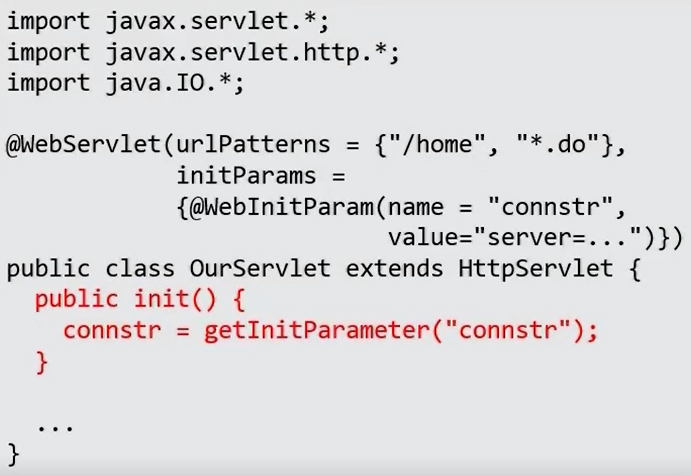
\includegraphics[width=7.5cm]{img/init_servlet.png}
		};
	\end{tikzpicture}
	\begin{itemize}
		\item Pour récupérer les données de connexion à un seveur de BdD, par ex
		\vspace{5cm}
		\item[] Possibilité de faire la même chose dans \texttt{web.xml}
	\end{itemize}
\end{frame}

\begin{frame}
	\frametitle{Initialiser toute l'application}
	\begin{tikzpicture}[overlay,remember picture]
		\node[anchor=center,xshift=0pt,yshift=0pt]
		at (current page.center) {
			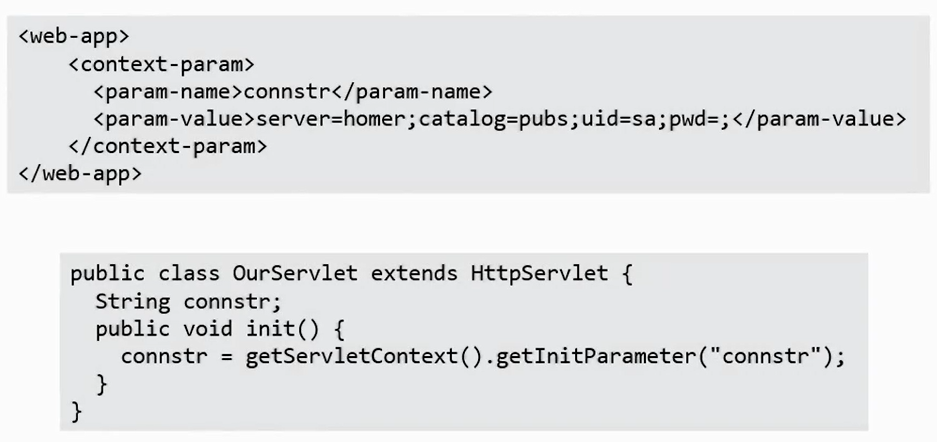
\includegraphics[width=10.5cm]{img/servlet_context.png}
		};
	\end{tikzpicture}
	\begin{itemize}
		\vspace{5cm}
		
		\item[]% Tester les deux solutions d'initialisation (par servlet et pour tout l'application)
	\end{itemize}
\end{frame}

\subsection{Jakarta Server Pages (JSP)}

\begin{frame}
	\frametitle{Architecture des applications JSP (Patron MVC)}
	\begin{tikzpicture}[overlay,remember picture]
		\node[anchor=center,xshift=0pt,yshift=-15pt]
		at (current page.center) {
			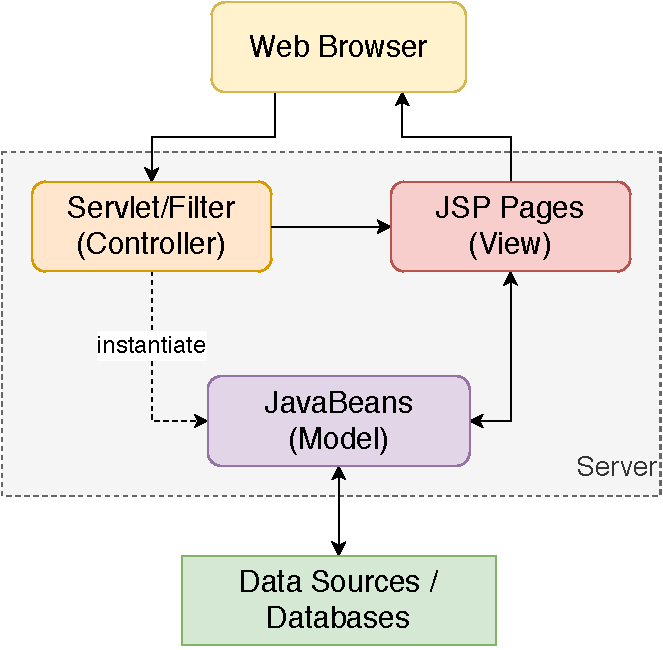
\includegraphics[width=7.5cm]{img/MVC_JSP.pdf}
		};
	\end{tikzpicture}
\end{frame}

\begin{frame}
  \frametitle{Pages JSP}
  \begin{itemize}
  	\item Mélange de code HTML et de code Java (éq. Php, ASP, ...)
  	\item Pages JSP transformées en servlets à l'exécution:
  	\begin{itemize}
  	\item Code source de la servlet généré puis compilé  lors de la réception de la première requête
  	\end{itemize}
  \item Scriptlet : balises \texttt{<\% et \%>}
    \begin{itemize}
    \item instructions Java exécutées pour réaliser des traitements
      lors de la réception d’une requête HTTP et pendant la
      fabrication de la réponse HTTP
    \end{itemize}
  \item Expressions : balises \texttt{<\%= et \%>}
    \begin{itemize}
    \item expression dont la valeur, convertie en chaîne, est incluse
      dans le flot HTML produit dans la réponse HTTP
    \end{itemize}
  \end{itemize}
\end{frame}

\begin{frame}
  \frametitle{Pages JSP -suite-}
    \begin{itemize}  
  \item Déclarations : balises \texttt{<\%! et \%>}
    \begin{itemize}
    \item déclaration de classe, de méthode, d’attribut, etc,
      utilisables dans les scriptlet et expressions précédentes
    \end{itemize}
  \item Directives d'inclusion : balises \texttt{<\%@ et \%>}
    \begin{itemize}
    \item directives d'inclusion de bibliothèques ou de fichiers (de code JSP)
    \end{itemize}
  \item Commentaires : balises \texttt{<\%-- et --\%>}
  \end{itemize}
\end{frame}

\begin{frame}
  \frametitle{Variables pré-définies et pré-initialisées dans les scripts}
    \begin{itemize}  
    \item \texttt{request} (HttpServletRequest) : objet correspondant
      à la requête HTTP (durée de vie = celle d’une seule interaction
      avec un client)
    \item \texttt{response} (HttpServletResponse) : objet réponse HTTP
    \item \texttt{out} (PrintWriter) : objet utilisé pour écrire dans
      le flot HTML de la réponse HTTP $\rightarrow$ \texttt{out.print(...);}
    \item \texttt{session} (HttpSession) : objet correspondant à la
      session (durée de vie = celle de la session avec un client)
    \item \texttt{application} (ServletContext) : objet 
      dont la durée de vie est égale à celle de l’application (initialisation de l'app)
    \item ...
  \end{itemize}
\end{frame}

\begin{frame}[fragile]
  \frametitle{Exemple de page JSP}
  \begin{flushleft}
  \begin{lstlisting}[language=HTML,basicstyle=\tiny]
<html>
  <head> <title>Converter</title> </head>
  <body>
    <h1><center>Converter</center></h1> <hr/>
    <p>Enter an amount to convert:</p>
    <form method="get">
      <input type="text" name="amount" size="25"> <br>
      <input type="submit" value="Submit"><input type="reset" value="Reset">
    </form>
    <% String amount = request.getParameter("amount");
    if ( amount != null && amount.length() > 0 ) {
      Double d = new Double (amount); %> <p>
      <%= amount %> dollars =
      <%= converter.dollarToYen(d.doubleValue()) %> Yen.</p><p>
      <%= amount %> Yen = <%= converter.yenToEuro(d.doubleValue()) %> Euro.
      </p>
    <% } %>
  </body>
</html>
\end{lstlisting}
  \end{flushleft}  
\end{frame}

\begin{frame}[fragile]
	\frametitle{A vos claviers -- reprendre l'app Web}
	\begin{itemize}
		\item Nous allons maintenant créer une page JSP qui affiche le message ``Hello'' suivi du nom de la personne
		\begin{itemize}
			\item ce qui correspond à la vue (on garde la servlet comme contrôleur)
		\end{itemize}
	\item Créer une page JSP (response.jsp) dans le dossier \texttt{webapp/}
	\item Ajouter dans le \textit{body} de cette page la ligne suivante~:\\
	\texttt{<h2>Hello, \$\{user\}!</h2>}\\
	D'où vient \texttt{\$\{user\}} ?
	\item C'est un attribut qui est inséré dans la requête HTTP qui est redirigée par la servlet~:
\begin{lstlisting}
String name = request.getParameter("name");
if (name == null) name = "World";
request.setAttribute("user", name);
request.getRequestDispatcher("response.jsp").forward(request, response);	
\end{lstlisting}
	\end{itemize}
\end{frame}


\begin{frame}[fragile]
	\frametitle{Gestion des erreurs dans JSP}
	\begin{itemize}
		\item Dans une section de code JAVA à l'intérieur d'une page JSP, on peut signaler une exception~:
		\begin{lstlisting}
if ( amount != null && amount.length() > 0 ) {
	...
}		
else {
	throw new ServletException("Il faut indiquer un montant");
}	
		\end{lstlisting}
		\item Qu'est-ce qu'on a sur le navigateur si une exception est levée ?
	\end{itemize}
\end{frame}

\begin{frame}
	\frametitle{Exception renvoyée au navigateur Web (par Jetty)}
	\begin{tikzpicture}[overlay,remember picture]
		\node[anchor=center,xshift=0pt,yshift=-15pt]
		at (current page.center) {
			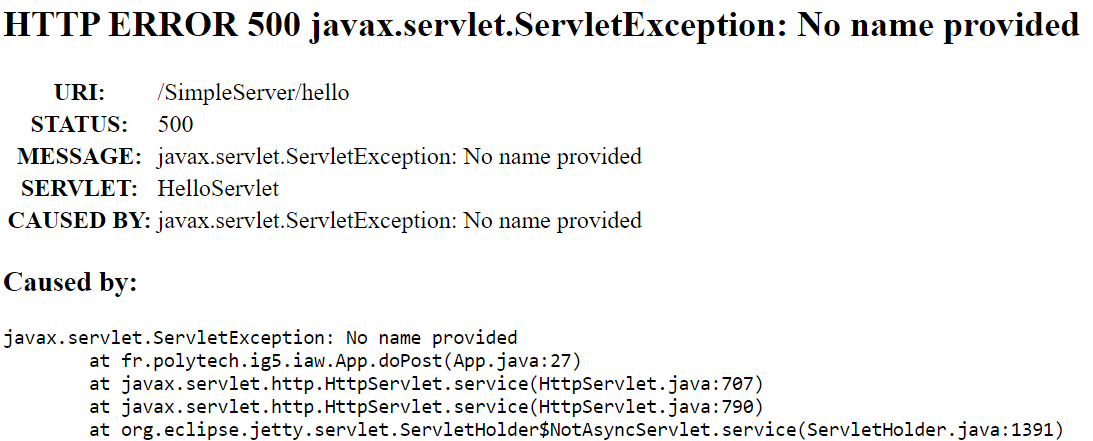
\includegraphics[width=10.5cm]{img/servlet_error.png}
		};
	\end{tikzpicture}
\end{frame}

\begin{frame}[fragile]
	\frametitle{Capturer l'exception et afficher une page d'erreur}
	\begin{itemize}
		\item D'abord, prévoir une redirection vers une page d'erreur dans web.xml
		\begin{lstlisting}[language=XML]
<error-page>
	<location>/error.jsp</location>
</error-page>		
		\end{lstlisting}
	\item Parenthèse~: on peut gérer plus finement les erreurs en ajoutant des pages d'erreurs spécifiques
\begin{lstlisting}
<error-page>
	<error-code>404</error-code>
	<location>/404.html</location>
</error-page>
\end{lstlisting}
	\end{itemize}
\end{frame}

\begin{frame}[fragile]
	\frametitle{Capturer l'exception et afficher une page d'erreur}
	\begin{itemize}
		\item Ensuite, créer la page \texttt{error.jsp} et dans cette page, on peut obtenir et afficher le message de l'exception
		\begin{lstlisting}[language=HTML]
<%@ page contentType="text/html;charset=UTF-8" 
 		language="java" %>
<%@ page isErrorPage="true" %>
<html>
  <head>
    <title>Error Page</title>
  </head>
  <body>
    <h2>Error Page!</h2>
	<%= exception.getMessage() %>
  </body>
</html>	
		\end{lstlisting}
		La directive "\texttt{page}" avec \texttt{isErrorPage="true"} donne accès à l'attribut \texttt{exception} (utilisé ci-dessus)
	\end{itemize}
\end{frame}

\begin{frame}
	\frametitle{A vos claviers -- reprendre l'app Web}
	\begin{itemize}
		\item Ajouter une page d'erreur si jamais un nom n'est pas fourni
		\item Tester à nouveau l'application
		\item Dans une vraie application Web, nous n'utilisons pas les exceptions pour ce genre de contrôles (c'est juste pour tester la gestion des erreurs ici)
	\end{itemize}
\end{frame}

\begin{frame}
	\frametitle{MVC avec des \textit{Servlet Dispatcher}}
	\begin{tikzpicture}[overlay,remember picture]
		\node[anchor=center,xshift=0pt,yshift=-15pt]
		at (current page.center) {
			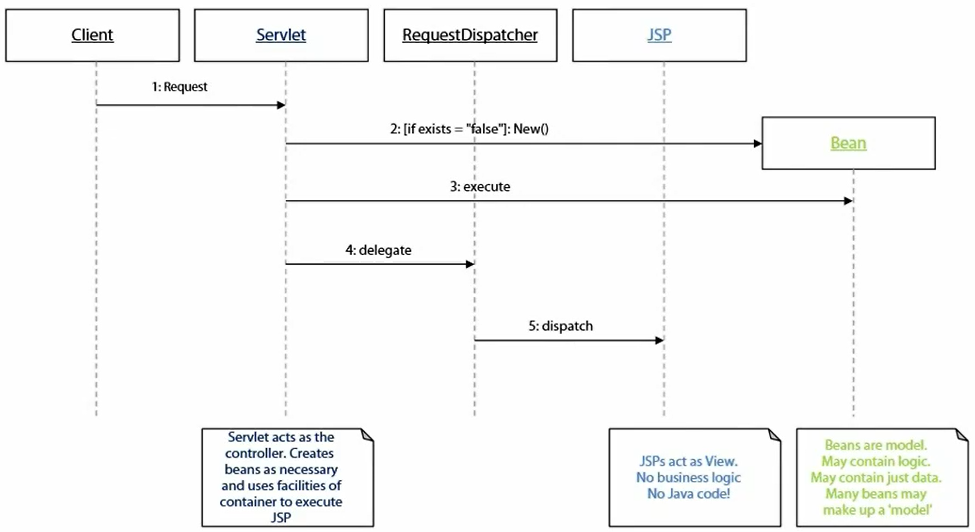
\includegraphics[width=12.5cm]{img/mvc_with_dispatcher.png}
		};
	\end{tikzpicture}
\end{frame}

\begin{frame}[fragile]
	\frametitle{MVC avec des \textit{Servlet Dispatcher} -suite-}
	\begin{itemize}
		\item Un objet \texttt{ServletDispatcher} peut être obtenu à partir du contexte de la servlet~: (extrait d'un précédent exemple)
\begin{lstlisting}
ServletDispatcher dispatcher = request.getRequestDispatcher("/response.jsp");
dispatcher.forward(request,response);
// ou bien dispatcher.include(request,response);
// qui permet de deleguer et ensuite reprendre la main
\end{lstlisting}
	\item Des objets (données) peuvent être inséré(e)s par la servlet (le contrôleur) avant de déléguer la requête
	\item Cette insertion se fait en invoquant la méthode \texttt{setAttribute("nom",valeur);} avant la délégation
	\item L'insertion de ces objets/données peut avoir plusieurs portées
	\end{itemize}
\end{frame}

\begin{frame}[fragile]
	\frametitle{Portées des objets/données dans une app Web}
	\begin{itemize}
		\item \textbf{Application} (durée de vie de toute l'application)~:
\begin{lstlisting}
getServletContext().setAttribute("db_server_url",url);
\end{lstlisting}
		\item \textbf{Session} (une session d'un utilisateur sur son navigateur -- plusieurs requêtes)~:
\begin{lstlisting}
getServletContext().getSession().setAttribute("user",user);	
\end{lstlisting}			
		Typiquement, c'est la portée qu'on utilise pour un panier dans une app de e-commerce 
		\item \textbf{Requête} (durée de vie de la requête HTTP)~:\\
\begin{lstlisting}
request.setAttribute("locale",locale);	
\end{lstlisting}					
	\end{itemize}
\end{frame}

\begin{frame}[fragile]
	\frametitle{Une dernière chose~: masquer les pages JSP}
	\begin{itemize}
		\item Essayer d'accéder à la page \url{http://localhost:8080/SimpleServer/error.jsp}\\
		Surprise !!!
		\item Déplacer les .jsp (avec refactoring) dans le dossier \texttt{WEB-INF/} (son contenu n'est pas rendu accessible par le serveur Web)
		\item S'assurer que toutes les références aux fichiers JSP sont correctes. Ex:\\
		\begin{lstlisting}
ServletDispatcher dispatcher = request.getRequestDispatcher("/WEB-INF/response.jsp");
		\end{lstlisting}
		\item Les pages JSP font partie de la vue (elles ne doivent pas être accessibles directement -- voir schéma du patron MVC)
	\end{itemize}
\end{frame}

\begin{frame}[fragile]
	\frametitle{Expression Language}
	\begin{itemize}
		\item Ce langage permet d'écrire des expressions qui permettent de réduire la quantité de code Java
		\item Syntaxe : une expression placée entre \texttt{\$\{} et \texttt{\}}
		\item Exemple : \texttt{<h2> Bienvenue \$\{user.name\} </h2>}\\
		ça récupère du contexte de la servlet (requête, session ou app) un objet \textit{JavaBean} user, puis exécute \texttt{user.getName()}~:
\begin{lstlisting}
<% User user = (User)request.getAttribute("user"); %>
<h2>Bienvenue <%= user.getName() %> </h2>		
\end{lstlisting}
C'est plus simple, non ?
\item On peut scripter du CSS également~:\\
\texttt{<div class=\$\{app.formCssClass.name\}></div>}
	\end{itemize}
\end{frame}

\begin{frame}
	\frametitle{Utiliser des JavaBeans et plein d'opérateurs dans JSP EL}
	\begin{itemize}
		\item Syntaxe JavaScript~: \texttt{user.name} ou \texttt{user["name"]}
		\item Opérateurs mathématiques~: +, -, *, /, \%
		\item Opérateurs de comparaison~: ==, !=, <, >, <=, >=
		\item Opérateurs logiques~: \&\&, ||, !
		\item Exemple~: \texttt{<h3>\$\{user.name == "Eva"\}</h3>}
		\item Opérateur vide~: permet de tester si une expression est égale à true, ou à une valeur différente de 0 ou null (selon son type), ça retourne la valeur true, sinon ça retourne false\\ 
		\texttt{\$\{!empty user.name\}} (éq. \texttt{user.name != null})
		
	\end{itemize}
Une dernière chose sur JSP~: vous savez ce qu'est JSTL~? Googler ce mot pour vous faire une idée
\end{frame}

\section{Écouteurs d'événements et filtres}

\subsection{Écouteurs -- \textit{Event Listeners}}
\begin{frame}
  \frametitle{Annotations}
  \begin{itemize}
  \item Les annotations remplacent parfois le code XML dans web.xml
  \item Seules les classes dans \texttt{WEB-INF/classes/} et les JAR dans \texttt{WEB-INF/lib/} sont scannés
  \item Nous avons déjà utilisé l'annotation \texttt{@WebServlet} pour remplacer une déclaration de servlet dans \texttt{web.xml}
  \item Nous pouvons déclarer des écouteurs en utilisant les annotations
  \end{itemize}
\end{frame}

\begin{frame}
	\frametitle{Qu'est-ce qu'un écouteur ?}
	\begin{itemize}
		\item Une section de code qui écoute un type d'événement particulier
		\item Utilisé souvent pour la journalisation -- \textit{logging} ou pour déclencher des traitements asynchrones
		\item Un événement est déclenché par le serveur à des moments précis de la vie d'une app Web~:
		\begin{itemize}
			\item Événements d'applications au démarrage/arrêt de l'app
			\item Événements de session au démarrage/arrêt d'une session
			\item Événements de requête au démarrage/arrêt d'une requête
			\item Événements d'attribut lors de l'ajout/suppression d'un attribut (au niveau App, Session ou Requête)
		\end{itemize}
	\end{itemize}
\end{frame}

\begin{frame}
	\frametitle{Comment définir un écouteur~?}
	\begin{itemize}
		\item Écrire une classe annotée par \texttt{WebListener} 
		\item Implémenter la bonne interface \texttt{Listener}~: \texttt{ServletContextListener} (app), \texttt{ServletContextAttributeListener} (attribut/app), \texttt{HttpSessionActivationListener} (session), \texttt{HttpSessionAttributeListener} (attribut/session), 
		\texttt{ServletRequestListener} (requête),
		\texttt{ServletRequestAttributeListener} (requête/attribut)
		\item Dans la classe ``écouteur d'évènement'', les méthodes callback à définir reçoivent en paramètre un objet ``évènement''
	\end{itemize}
\end{frame}

\begin{frame}
	\frametitle{Exemple d'écouteur d'évènements d'application}
	\begin{tikzpicture}[overlay,remember picture]
		\node[anchor=center,xshift=0pt,yshift=5pt]
		at (current page.center) {
			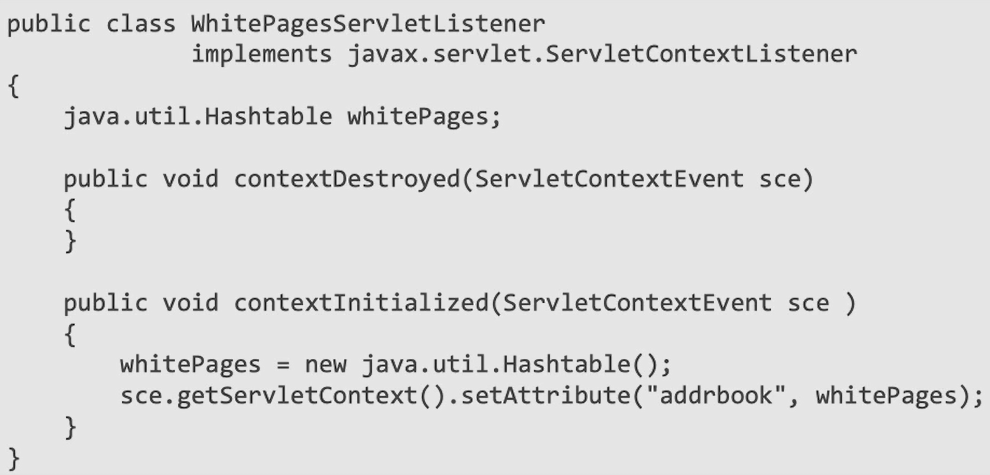
\includegraphics[width=12cm]{img/app_listener.png}
		};
	\end{tikzpicture}
\begin{itemize}
	
\vspace{5cm}

\item Il est possible d'étendre la classe Adapter ``\texttt{EventListener}'' pour ne pas devoir implémenter toutes les méthodes abstraites

\end{itemize}
\end{frame}

\begin{frame}[fragile]
	\frametitle{Un écouteur d'événements liés aux attributs d'une session}
	\begin{itemize}
		\item D'abord, la durée d'une session peut être paramétrée. Dans \texttt{web.xml}~:
\begin{lstlisting}
<session-config>
	<session-timeout>1</session-timeout>
</session-config>		
\end{lstlisting}
La durée est exprimée en minutes ici
\item L'objet événement de type \texttt{HttpSessionEvent} fournit une méthode \texttt{getSession()} qui permet d'obtenir le contexte de la servlet (méthode \texttt{getServletContext()}). Ce dernier objet permet de faire des logs~:\\
\footnotesize
\texttt{event.getSession().getServletContext().log("Session utilisateur démarrée);}
\normalsize
	\end{itemize}
\end{frame}

\subsection{Filtres}
\begin{frame}
  \frametitle{Qu'est-ce qu'un filtre}
  \begin{itemize}
  \item Une section de code qui intercepte une requête et qui effectue dessus un traitement supplémentaire~:
  \begin{itemize}
  	\item Ils sont exécutés avant/après l'exécution d'une requête
  	\item La requête peut être pour une page HTML, page JSP, une servlet, ...
  	\item La requête et la réponse peuvent être modifiées
  	\item Les filtres peuvent être exécutées en chaîne
  	\item Les filtres peuvent intercepter la requête originale des \texttt{forward} et \texttt{include} (voir \texttt{ServletDispatcher})
  	\item Les filtres sont utilisés pour gérer des sessions, la journalisation (\textit{logging}), la sécurité, ...
  \end{itemize}
  \end{itemize}
\end{frame}

\begin{frame}
	\frametitle{Chaîne de filtres (synchrones -- appels bloquants)}
	\begin{tikzpicture}[overlay,remember picture]
		\node[anchor=center,xshift=0pt,yshift=5pt]
		at (current page.center) {
			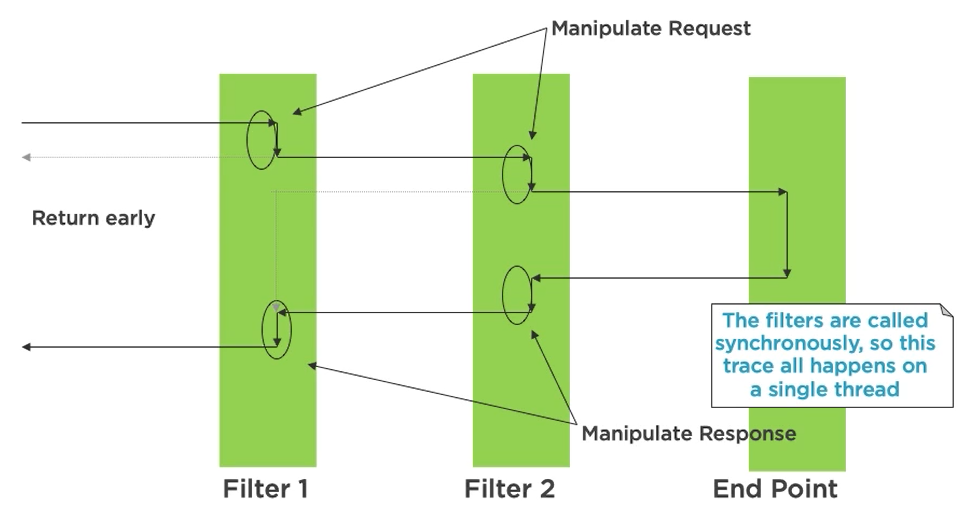
\includegraphics[width=10cm]{img/filter_chain.png}
		};
	\end{tikzpicture}
	\begin{itemize}
		\vspace{5cm}
		\item Le filtre 1 peut être un filtre de sécurité, qui ne laisse pas passer la requête si utilisateur non-authentifié/autorisé
		\item Le filtre 2 peut gérer le \textit{logging} par exemple
	\end{itemize}
\end{frame}

\begin{frame}[fragile]
\frametitle{Comment définir un filtre~?}
	\begin{itemize}
		\item Une classe qui implémente l'interface \texttt{javax.servlet.Filter}~:
\begin{lstlisting}
// Called once at start
public void init(FilterConfig config);
// Called once at end
public void destroy(FilterConfig config);
// where the work is done
public void doFilter(ServletRequest request,
                     ServletResponse response,
                     FilterChain chain);
\end{lstlisting}
\item Appeler \texttt{chain.doFilter(...)} pour continuer l'exécution de la chaine de filtres 
	\end{itemize}
\end{frame}

\begin{frame}
	\frametitle{Configuration d'un filtre}
	\begin{tikzpicture}[overlay,remember picture]
		\node[anchor=center,xshift=0pt,yshift=5pt]
		at (current page.center) {
			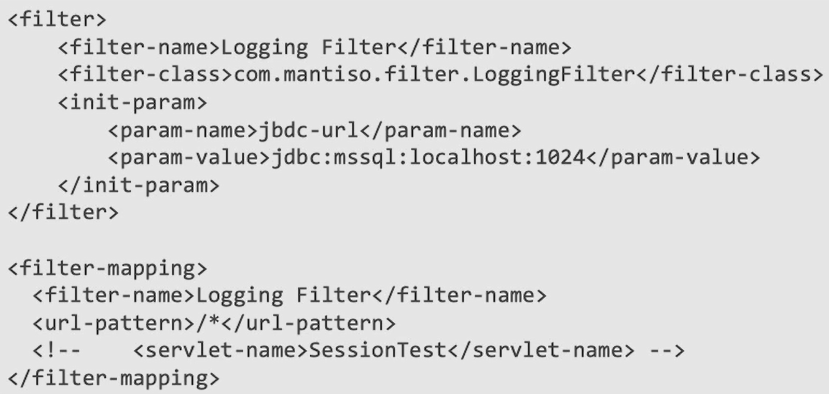
\includegraphics[width=10cm]{img/filter_config.png}
		};
	\end{tikzpicture}
	\begin{itemize}
		\vspace{5cm}
		\item Les filtres peuvent être associés à une ressource ou un URL
		\item Possible de le faire avec des annotations~: \texttt{@WebFilter(urlPatterns="*.do")}
		et \texttt{@WebInitParam}
	\end{itemize}
\end{frame}

\begin{frame}
	\frametitle{Structure-type d'un filtre}
	\begin{tikzpicture}[overlay,remember picture]
		\node[anchor=center,xshift=0pt,yshift=-15pt]
		at (current page.center) {
			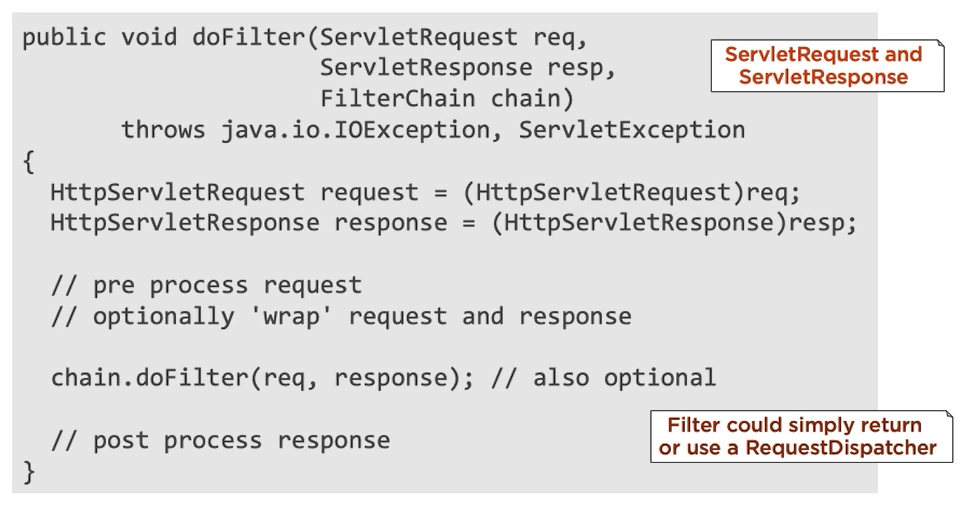
\includegraphics[width=12cm]{img/do_filter.png}
		};
	\end{tikzpicture}	
\end{frame}

\begin{frame}
	\frametitle{Wrappers des requêtes et réponses HTTP}
	\begin{itemize}
		\item Dans certains cas, on est amené à écrire des wrappers pour les requêtes ou les réponses HTTP
		\item Ce sont des classes, qui étendent des classes Adapter (\texttt{HttpServletRequestWrapper} ou \texttt{HttpServletResponseWrapper}) pour~:
		\begin{itemize}
			\item utiliser une journalisation log4j de certaines informations dans les requêtes
			\item transformer ou compresser les réponses 
			\item ...
		\end{itemize}
	\end{itemize}
\end{frame}

\section{Servlets asynchrones}
\begin{frame}
	\frametitle{Pourquoi on recherche parfois l'asynchronisme~?}
	\begin{itemize}
		\item Lorsqu'on a des traitements au backend qui peuvent être lents (invocation d'un service externe lent)
		\item Lorsque l'on fait des entrées/sorties dans le backend qui peuvent bloquer (la tendance maintenant dans la plupart des API est au NIO -- \textit{Non-blocking IO}, par défaut)
		\item Pour permettre au serveur Web de réutiliser le thread d'accueil des requêtes du client (en réalité, il y en a plusieurs, des \textit{HTTP worker threads}. Tomcat peut en créer jusqu'à 200, valeur par défaut)
		\item Pour permettre le ``\textit{Server Push}'': le serveur peut notifier les clients, qui font du ``\textit{long polling}'', d'informations qui sont mises à jour régulièrement (réseaux sociaux, ...)
	\end{itemize}
L'objectif ultime est rendre une application Web \textbf{scalable}
\end{frame}

\begin{frame}
	\frametitle{Mode d'emploi des servlets asynchrones}
	\begin{enumerate}
		\item Démarrer un contexte de servlet asynchrone en utilisant l'objet représentant la requête HTTP
		\item Utiliser ce contexte pour accéder à la requête et retourner la réponse, mais en effectuant cela dans un thread à part,  afin de libérer le thread worker (HTTP) du serveur
		\item Éventuellement, ajouter des écouteurs au contexte pour gérer les événements (timeout, ...)
		\item Indiquer la fin du contexte asynchrone pour déclencher le renvoi de la réponse au client
	\end{enumerate}
On peut définir des filtres asynchrones également (non présentés ici)
\end{frame}

\begin{frame}[fragile]
	\frametitle{Écrire une servlet asynchrone}
	\begin{itemize}
		\item D'abord annoter la servlet comme asynchrone~:
\begin{lstlisting}
@WebServlet(urlPatterns="/home", asyncSupported=true)
public class FirstAsyncServlet extends HttpServlet {
}
\end{lstlisting}
\item Démarrer le contexte de servlet asynchrone~:
\begin{lstlisting}
@Override
public void doGet(HttpServletRequest request,
                  HttpServletResponse response) {
	final AsyncContext ctx = req.startAsync();
	// ...
}
\end{lstlisting}
L'invocation de \texttt{startAsync()} indique au serveur que la réponse ne doit pas être retournée au client à la fin du \texttt{doGet(...)}
	\end{itemize}
\end{frame}

\begin{frame}[fragile]
	\frametitle{Écrire une servlet asynchrone -suite-}
	\begin{itemize}
		\item Démarrer et arrêter le traitement asynchrone dans un autre thread~:
\begin{lstlisting}
ctx.start(() -> {
	try { // ...
		ctx.getResponse().getWriter().write(...);
	}
	catch(IOException e) {
		log("Un probleme est survenu lors du traitement asynchrone",e);
	}
	ctx.complete();
});
\end{lstlisting}
\item Autre possibilité~: déléguer le traitement à une autre servlet
\begin{lstlisting}
final AsyncContext ctx = req.startAsync();
ctx.dispatch("/uneUrl");
\end{lstlisting}
	\end{itemize}
\end{frame}

\begin{frame}[fragile]
	\frametitle{Fin du traitement asynchrone}
	\begin{itemize}
		\item Possibilité de définir un timeout pour une servlet asynchrone
		\item Fixer la durée du timeout~:
\begin{lstlisting}
ctx.setTimeout(5 * 1000); // temps en millisecondes 
\end{lstlisting}
	\item A la fin, indiquer que le traitement de la requête asynchrone est terminé : \texttt{ctx.complete();}
	\end{itemize}
\end{frame}

\begin{frame}
	\frametitle{Ecouteurs d'événements pour une servlet asynchrone}
	\begin{tikzpicture}[overlay,remember picture]
		\node[anchor=center,xshift=0pt,yshift=0pt]
		at (current page.center) {
			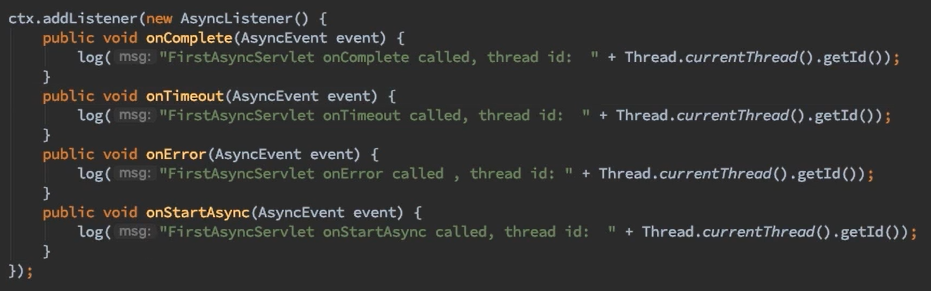
\includegraphics[width=12cm]{img/listeners_async_servlet.png}
		};
	\end{tikzpicture}
\end{frame}

\begin{frame}
	\frametitle{A vos claviers}
	\begin{itemize}
		\item Faire le sujet de TP sur le dépôt Git, après avoir visionné les derniers slides
	\end{itemize}
\end{frame}

\section{Conclusion}

\begin{frame}
  \frametitle{Présence de Java dans le back-end de grandes app Web (Source~: Wikipedia, Oct. 2021)}
  \begin{tikzpicture}[overlay,remember picture]
    \node[anchor=center,xshift=0pt,yshift=-15pt]
    at (current page.center) {
      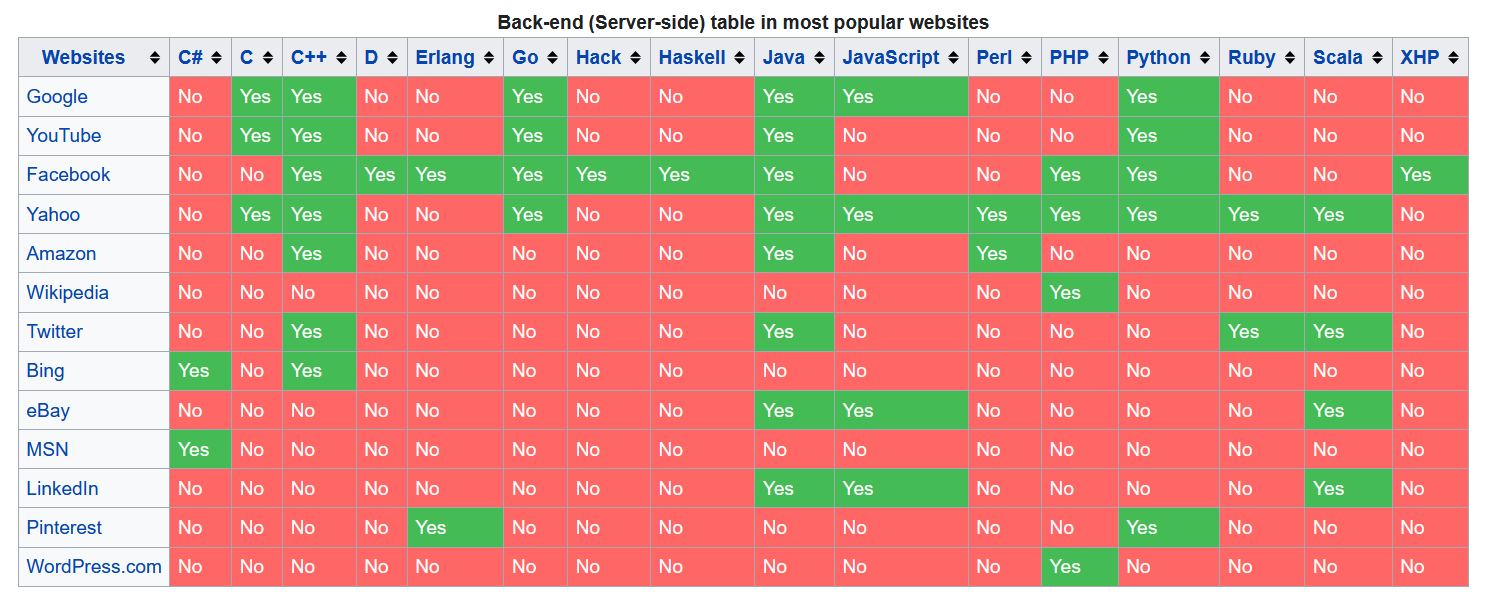
\includegraphics[width=12cm]{img/server_side_java.png}
    };
  \end{tikzpicture}
\begin{itemize}
\vspace{5cm}
\item[] Présent dans le plus grand nombre de ces grandes app Web (+~Netflix, ...)
\end{itemize}
\end{frame} 

\begin{frame}
	\frametitle{\textit{Wrap-up}}
	\begin{itemize}
		\item Programmation de back-end (et un peu de Front) d'applications Web en Java 
		\item Back-end structuré, qui profite des forces de la prog par objets et des design patterns associés
		\item Programmation avec un langage à typage statique (détecter certaines erreurs, de typage notamment, au plus tôt)
		\item Mécanisme déclaratif (à base d'annotations) pour la définition de filtres, d'écouteurs d'événements, de servlets asynchrones, ...
		\item Scalabilité d'une appli Web grâce aux servlets asynchrones
		\item Prochains cours : framework qui exploite toutes les notions de ce cours et rend leur utilisation plus simple
	\end{itemize}
\end{frame}

\begin{frame}
      \begin{tikzpicture}[overlay,remember picture]
        \node[anchor=center,xshift=0pt,yshift=20pt]
        at (current page.center) {
          
\includegraphics[width=4cm]{img/question.jpg}
        };
      \end{tikzpicture}
  \begin{center}
  
  	\vspace{5cm}
  	
  	Vous pouvez envoyer vos questions\\ ou commentaires par mail
  \end{center}
\end{frame}

\end{document}
